Die Nutzung von EC2-Instanzen ist mit einem Zahlungsmodell verbunden. Die Wahl des Zahlungsmodells ist von entscheidender Bedeutung, um den besten Preis für EC2-Instanzen zu erzielen.
%EC2 and RDS(DB) spend are often on of the main portions of your overall AWS Bill t.ly/Mqwn
Die von Amazon Web Services angebotenen Zahlungsmodelle werden im Folgenden dargestellt.
\\\\
Das On-Demand-Modell beinhaltet keine langfristigen Verpflichtungen, es ist daher die teuerste Alternative, die auf Stundenbasis berechnet wird. Die Modelle Saving Plans und Reserved Instances erfordern den Abschluss von Verträgen über ein oder drei Jahre, um günstige Preise zu erhalten. EC2-Spot-Instanzen sind das kostengünstigste Modell, sie haben aber den Nachteil, dass ihre Verfügbarkeit nicht immer garantiert ist. Jedes Zahlungsmodell hat seine Vor- und Nachteile und eignet sich für unterschiedliche Anwendungsfälle. Gute Ergebnisse können auch durch die Kombination mehrerer Zahlungsmodelle erzielt werden[ZU ERGÄNZEN]. %SAG DER CLOUD-EXPERT/FIRMA
Dies wird in Unterkapitel \ref{sssec:num2.4} behandelt.
%[WIRD ES?]
\\\\
In dieser Arbeit wird nicht darauf eingegangen, wie die richtige Server-Instanz ausgewählt werden sollte, da die Auswahl von individuellen Anforderungen abhängt, die von Fall zu Fall unterschiedlich sind. Im Allgemeinen wird empfohlen Instanzen so nahe wie möglich an den Ressourcen, mit denen sie kommunizieren werden, zu platzieren. %[IST DIESE ERKLÄRUNG NÖTIG?]
% Ressourcen vs Cloud-Dienste sollte gekläert werden
Die beste Leistung wird außerdem angestrebt, indem sich diese Instanzen in räumlicher Nähe zur Mehrzahl der Endnutzer, befinden. 
%Vor- und Nachteile noch tabellarisch aufzulisten??
%https://youtu.be/Q5wSvUVPyYY?t=678
%Excess capacity/Spot Instances
\subsection{On-Demand-Instanzen}
Bei diesem Zahlungsmodell besteht keine Notwendigkeit, ein festes Anfangsbudget festzulegen. Die Kosten richten sich nach dem Verbrauch auf der Grundlage der Nutzungsstunden. Dieses Modell eignet sich für Projekte, deren Entwicklung unvorhersehbar ist und die Möglichkeit besteht, dass das es in kurzer Zeit abgeschlossen sein wird, sodass es nicht Sinnvoll ist, eine langfristige Verpflichtung einzugehen.
\\\\
Die Preise beim dem On-Demand Zahlungsmodell variiert je nach Instanz Typ, Region und der übertragenen Datenmenge. Die aktuellen Preise für die verschiedenen Regionen sind auf der Amazon-Website in der Sektion EC2 - On-Demand-Preise\footnote{\cite{AMZ02}AWS On-Demand Instances Pricing} zu finden. 
%Hierzu ein Beispiel für die Preise der EC2-Instanzen im On-Demand Zahlungsmodell.
\begin{figure}
    \centering
    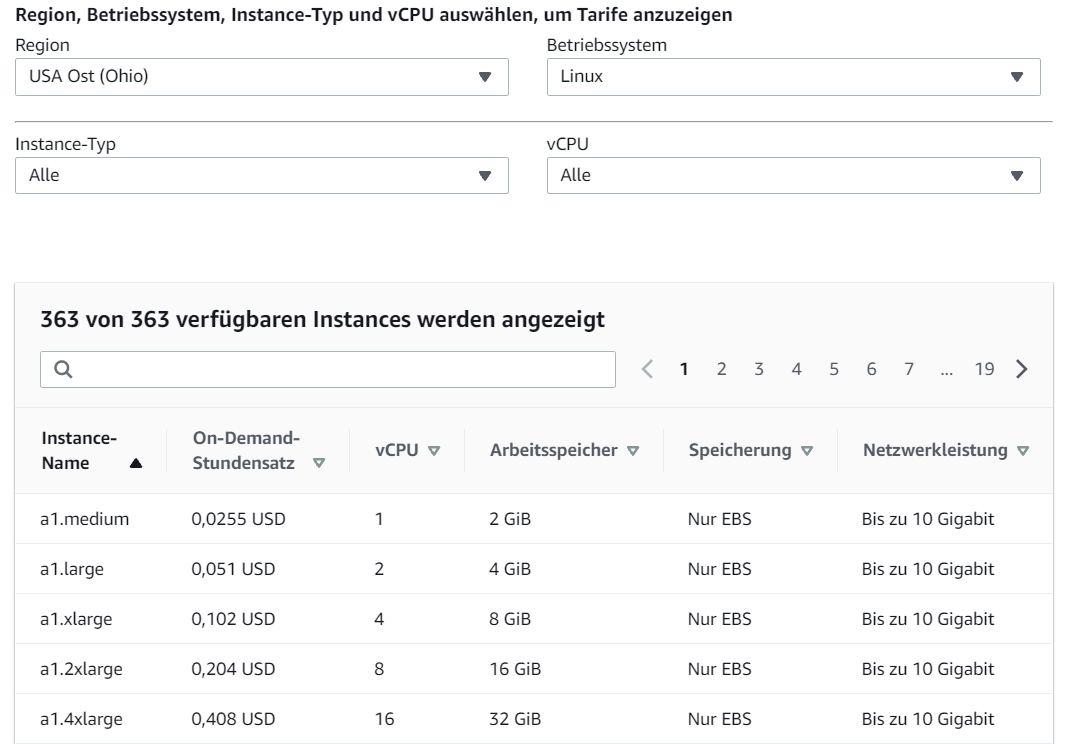
\includegraphics[scale=0.5]{sources/On-Demand-Pläne für Amazon EC2}\label{fig:OnDemand_Preise}\\
    \caption[On-Demand Preise für Amazon EC2]{}
    \label{fig:OnDemand_Preise}  On-Demand Preise für Amazon EC2 \footnote{\cite{AMZ02}}
  \end{figure}
In der \autoref{fig:OnDemand_Preise} werden die für die Region Ohio verfügbaren Linux-Instanzen gezeigt. Es ist zu beachten, dass Instanzen mit denselben Eigenschaften, aber in verschiedenen Regionen, unterschiedliche Preise haben können.
 %WARUM IST DIESE ABB.?
\subsection{Reservierte Instanzen und Saving Plans}
%t.ly/JUWq
%https://www.youtube.com/watch?v=c_zlPQimrvY
Die Zahlungsmodelle Reservierte Instanzen und Saving Plans sind sich sehr ähnlich. Beide kommen mit einer gleichbleibenden  Nutzungsverpflichtung, die in €/Stunden gemessen wird. Um die reduzierten Preise  zu bekommen, müssen Verträge über ein oder drei Jahre abgeschlossen werden. 
\\\\
Die \autoref{fig:EinsparungenRISP} zeigt die möglichen Einsparungen je nach Zahlungsmodell. Die Einsparungen hängen mit der Flexibilität bei der Wahl der Instanzfamilie und der Verfügbarkeitszone zusammen, in die Instanzen übertragen werden können. Je geringer die Flexibilität, desto höher die Einsparungen.
\begin{figure}[h!]
  \centering
  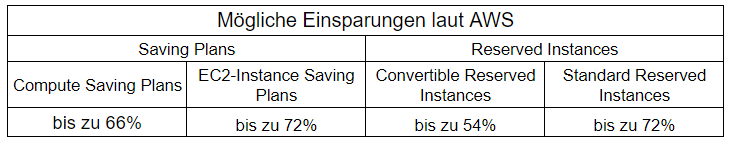
\includegraphics[scale=0.8]{sources/EinsparungenRISP}\label{fig:EinsparungenRISP}\\
  \caption[Mögliche Einsparungen bei Reserved Instances and Saving Plans laut AWS]{}
  \label{fig:EinsparungenRISP}
  Mögliche Einsparungen bei Reserved Instances and Saving Plans laut AWS
  \footnote{\cite{AMZ07,AMZ11}}
\end{figure}
\\
Compute Saving Plans\footnote{\cite{AMZ11}AWS Saving Plans Pricing} bieten die Flexibilität EC2-Instanzen nach Familie\footnote{\cite{AWS1},WS Certified Solutions Architect - Associate (SAA-C02), Seite 95}, Größe, Verfügbarkeitszone (AZ), Betriebssystem oder Mandant zu wechseln. Diese Option ist bei EC2-Instance Saving nicht möglich und daher bietet diese Alternative eine etwas höher Einsparung.
\begin{quote}
    „Bei Compute Saving Plans können Sie beispielsweise jederzeit von C4- auf M5-Instances wechseln, eine Workload von EU (Irland) nach EU (London) verlagern oder eine Workload von EC2 auf Fargate oder Lambda verschieben. Dabei zahlen Sie automatisch weiterhin den Saving Plans-Preis.”
    \footnote{\cite{AMZ11}AWS Saving Plans Pricing}
\end{quote}
Bei den EC2-Instance Saving Plans hingegen muss eine Instance-Familie in einer bestimmten Region ausgewählt werden.  Dies reduziert automatisch die Kosten für die ausgewählte Instanz-Familie in der jeweiligen Region, unabhängig von Availability Zone, Größe, Betriebssystem oder Mandant.
%\\Die Festlegung eines festen Stundensatzes über einen langen Zeitraum bietet die Möglichkeit, künftige Kosten zu planen[ZITAT/WIE IM BWL ERKLÄRT]WIEDER EINBLENDEN; WENN ES SINNVOLL IST.
%-
%Folgenden Kriterien definieren den Preis von EC2-Instanzen bei SavingPlans:
%Vertraglaufzeit, Vorabzahlung, Betriebssystem,Region, Mandant
%AUCH FÜR RIs?
%3 Arten von S. Plans: Compute and EC2 Instance
\subsubsection*{EC2 Reserved Instance Marketplace}\label{sssec:RI-Marketplace}
Sollte sich herausstellen, dass die Kapazität der reservierten Instanzen viel zu wenig oder gar nicht genutzt wird, kann diese Rechenkapazität auf dem RI Marketplace zur Verfügung gestellt werden. Dadurch könnte Teil der Investition wieder hereinzuholen. Dies ist für Standard Reserved Instances möglich. Diese Instanzen werden in Spot-Instanzen umgewandelt damit andere Nutzer sie beantragen können. Eine Servicegebühr sollte in Betracht gezogen werden. Im November 2021 beträgt diese Abgabe 12\%\footnote{\cite{AMZ23}Amazon EC2 Reserved Instance Marketplace}.[Rev]

\subsubsection*{Vorauszahlung}\label{sssec:Vorauszahlung}
Zusätzlich gibt es bei Saving Plans und reservierten Instanzen die Option im Voraus zu zahlen. Im Gegenzug wird ein niedrigerer Preis angeboten. Amazon bietet drei verschiedene Optionen an. Diese sind teilweise, keine oder vollständige Vorauszahlung\footnote{\cite{AMZ17} AWS Pricing Calculator}. Bei teilweiser Vorauszahlung ist eine Anzahlung von etwa 50\% zu leisten.
\\\\
Die \autoref{fig:EinsparungenVorauszahlung} zeigt den Vergleich zwischen den drei Optionen für Vorauszahlungen. Hier wird deutlich, dass es kaum einen Unterschied zwischen eine teilweise Vorauszahlung und keine Vorauszahlung zu machen gibt. Eine erhebliche Einsparung ergibt sich, wenn man für den gesamten Zeitraum der gebuchten Instanzen im Voraus bezahlt.
\begin{figure}[h!]
    \centering
    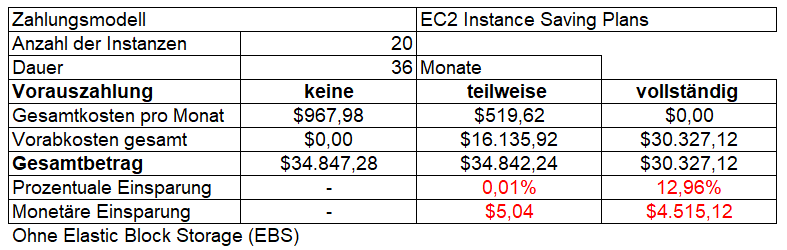
\includegraphics[scale=0.6]{sources/EinsparungenVorauszahlung}\label{fig:EinsparungenVorauszahlung}\\
    \caption[Mögliche Einsparungen durch Vorauszahlungen]{}
    \label{fig:EinsparungenVorauszahlung}Mögliche Einsparungen durch Vorauszahlungen für EC2 Instanzen in Saving Plans Zahlungsmodell\\
    Eigene Darstellung. Quelle: {\cite{AMZ17}AWS Pricing Calculator}
  \end{figure}
  \\
Die Berechnungen wurden mit dem AWS Pricing Calculator {\cite{AMZ17}} für Instanzen der Familie t4g.xlarge, in der EU (Frankfurt) und für eine Laufzeit von 3 Jahren durchgeführt. 
\subsection{Spot Instanzen }\label{ssec:Spot-Instances}
Wie in Unterkapitel \ref{sssec:RI-Marketplace} genannt bieten EC2 Spot-Instanzen die Möglichkeit aus den ungenutzten EC2-Instanzen anderer Nutzer zu profitieren. 
Mit einem Preisvorteil von bis zu 90 \% gegenüber normalen On-Demand-Instanzen sind Spot-Instanzen ideal für fehlertolerante Anwendungen wie auf Containern ausgeführte Workloads, CI/CD, Bigdata-Anwendungen und ähnliches.

\subsubsection*{Unterbrechbarkeit}
Es ist zu beachten, dass Spot-Instanzen jederzeit unterbrochen werden können. Einer der Gründe ist die Preisüberschreitung der Instanz. Wenn Spot-Instanzen angefordert werden, wird einen Maximalpreis festgelegt. Ist der Preis der Spot-Instanz höher als der eingegebene Maximalpreis, ist die Spot-Instanz für die aktuelle Einstellung nicht mehr verfügbar. Ein anderes Szenario ist, wenn der Instanz Anbieter die Spot-Instanz erneut anfordert. Falls eine Spot-Instanz unterbrochen wird, benachrichtigt Amazon EC2 zwei Minuten im Voraus. Dieses Ereignis ist verfügbar auf CloudWatch, damit weitere Alarmen eingestellt werden. Diese und andere Funktionalitäten von CloudWatch werden in Kapitel \ref{kap_kostenüberwachung } näher erläutert.
\\
Da Spot-Instanzen anfällig für Unterbrechungen sind, ist es nicht empfehlenswert, für Produktionsumgebungen nur Spot-Instanzen zu verwenden.
%Um von der Preisvorteile der Spot-Instanzen zu profitieren und Ausfälle zu vermeiden, sollten in Kombination weitere Zahlungsmodelle verwenden werden.
%\\
%Zum Beispiel eine Kombination aus Spot-Instanzen für die erwarteten Last und On-Demand-Instanzen für die dynamischen Last.
%https://aws.amazon.com/de/ec2/spot/pricing/

%2 OPTIONEN: LOWEST PRICE OR DIVERSIFIED ACROSS n POOLS TO AVOID DOWNS https://www.linkedin.com/learning/aws-automation-and-optimization/request-spot-instances-part-2?autoAdvance=true&autoSkip=true&autoplay=true&resume=false&u=79182202
\subsection{Wahl des Zahlungsmodells} \label{sssec:num2.4}
%Vor- und Nachteile? 
Die Reservierung von Instanzen mit Plänen, die zu zeitlichen Verpflichtungen führen, birgt die Gefahr, dass die benötigte Rechenkapazität langfristig falsch eingeschätzt wird. 
%A continuacion dos casos. En uno la capacidad de computo es muy baja y se necesita mucha capacidad de instancias On-Demand. En la segunda la capacidad de intancias reservadas es demasiada y haber usado instancias On-Demand hubiera sido en total mas economico.
Hier sind zwei Fälle. In einem Fall ist die Rechnerkapazität sehr gering und es wird viel On-Demand-Instanzkapazität benötigt. Im zweiten Fall ist die reservierte Instanzkapazität zu hoch und die Verwendung von On-Demand-Instanzen wäre insgesamt rentabler gewesen.
%SHOW THIS
%https://medium.com/driven-by-code/how-truecar-saves-40-on-aws-with-ec2-reserved-instances-d0a6e0d9c08a
[How TrueCar Saves 40\% on AWS with EC2 Reserved Instances]

\subsection{Amazon EC2 Fleet[rev]} \label{sssec:AWS-EC2-Fleet}
Instanzen-Flotte oder auf Englisch fleet of instances, bieten bei AWS die Möglichkeit mehrere Spot-Instanzen anzufordern, um einen bestimmten Bedarf an Rechenleistung zu decken\footnote{\cite{AMZ26} Amazon Elastic Compute Cloud - Benutzerhandbuch für Linux-Instances, Seite 708}. Spot-Instanzen können auch für produktive Umgebungen verwendet werden\footnote{\cite{AMZ24} Running Web Applications on Amazon EC2 Spot Instances}. Darüber hinaus ist es empfehlenswert, Instanzen aus verschiedenen Zahlungsmodellen zu kombinieren, um von den Einsparungen von Spot-Instanzen, Saving Plans und reservierten Instanzen zu profitieren. Die Kombination von Instanzen aus verschiedenen Zahlungsmodellen beseitigt den Nachteil für Produktionsumgebungen, der mit Spot-Instanzen verbunden ist. Das heißt, das Risiko eines vollständigen oder teilweisen Ausfalls der Rechenkapazität durch den Ausfall von Spot-Instanzen stellt.
\\\\
Folgende Punkte sind für die Nutzung von Spot Fleet Instanzen zu berücksichtigen:
\subsubsection*{Wahl der Instanzen[rev]}
Die Instanzen, die in der Auswahl für die Instanzen-Flotte berücksichtigt werden, müssen die Anforderungen der Applikation entsprechen. Um die Wahrscheinlichkeit zu erhöhen, dass Spot-Instanzen gefunden werden, ist es empfehlenswert, die Kriterien der Suche zu erweitern in dem man Instanzen ähnlicher Typen zulässt. Die Berücksichtigung von Instanzen von Familien mit mehr Leistung als erforderlich ist ebenfalls eine gute Option. Denn, obwohl die Leistung die Anforderungen der Applikation überstiegen werden, wird es einen reduzierten Preis für die Spot-Instanzen bezahlt als bei On-Demand Zahlungsmodell.
\\\\
\subsubsection*{Maximaler Stundenpreis[rev]}
Wie im Unterkapitel \ref{ssec:Spot-Instances} erwähnt, muss für Anforderung von Spot-Instanzen einen Maximalpreis festlegt werden. In diesem Fall ist die Festlegung dieses Maximalpreises auch für die gesamte Instanzen-Flotte eine Option. Es kann erwartet werden, dass die Spot-Preise im Laufe der Zeit stabil bleiben, das heißt keine starke Preisschwankungen. Der aktuelle Preis und der Preisverlauf von Spot-Instanzen können in auf dem AWS-Konsole\footnote{\cite{AMZ25} AWS EC2 Spot Instanzen-Anfragen und Preisverlauf} abgefragt werden. Diese Informationen sind zugänglich nur mit einem AWS-Konto.
\\
\subsubsection*{Festlegung von On-Demand-Anteil[rev]}
Die Standardeinstellungen sind ein guter Ausgangspunkt und liegen bei 70\% On-Demand-Instanzen und 30\% Spot-Instanzen.
\cite{AMZ24}

\subsubsection*{Auto Scaling group[rev]}
\subsubsection*{Einschränkungen[rev]}


\subsection*{Vergleich der Zahlungsmodelle}
Die folgende Tabelle fasst die Eigenschaften der Zahlungsmodelle für EC2-Instanzen zusammen und listet typische Applikationen je nach Zahlungsmodell auf.
[Abb. VOLLSTÄNDIG?]
\begin{figure}[h!]
    \centering
    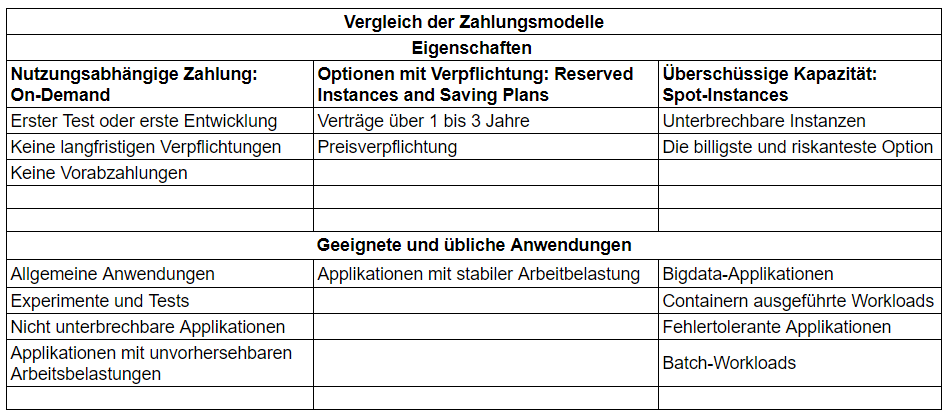
\includegraphics[scale=0.63]{sources/Vergleich_der_Zahlungsmodelle}\label{fig:Vergleich_der_Zahlungsmodelle}\\
    \caption[Vergleich der Zahlungsmodelle]{}
    \label{fig:Vergleich_der_Zahlungsmodelle}  Vergleich der Zahlungsmodelle nach Eingenschaft und Anwendungsfall\\
Eigene Darstellung. Quelle: {\cite{AMZ02, AMZ07, AMZ11, AMZ19,SPOT1}}\\
{\cite{PS1}Plusserver: Kostenoptimierung in AWS Seite 9}
  \end{figure}
%
%To read planned at 21.11:
%https://www.pcapps.com/services/aws-reserved-vs-on-demand-instances/
%https://jaychapel.medium.com/aws-reserved-instances-versus-on-demand-which-is-better-e7f77f1f9582
%https://www.cloudhealthtech.com/blog/aws-reserved-instances-vs-on-demand#:~:text=In%20terms%20of%20compute%20options,of%20an%20On%20Demand%20instance.
%https://youtu.be/mKEdhmJ2udA?t=79
%Automate the selection to get the best price
%https://spot.io/aws-cost-optimization-calculator/
\\\\
\subsubsection*{Fazit}
In diesem Kapitel wurden die verschiedenen Zahlungsmodelle für EC2-Instanzen untersucht. Es wurden Hinweise für die Auswahl des richtigen Zahlungsmodells in verschiedenen Szenarien gegeben. Dies wurde erklärt, um die Preisvorteile von den Zahlungsmodellen zu nutzen. Beginnend mit dem On-Demand-Zahlungsmodell, gefolgt von Reserved Instanzen und Saving Plans. In dieser Reihenfolge sinkt der Preis und mit ihm steigt die Verpflichtung, sich langfristig zu binden. Schließlich mit Spot-Instanzen, die die niedrigsten Preise bieten, aber keine volle Verfügbarkeit sicherstellen.%oder garantieren?
\\\\
%En el capitulo monitoreo de costes  se mostrarán herramientas como X(CloudWatch) con las que podremos verificar si la desicion realizada fue la correcta. Para el modelo de pago On-Demand no hay ninguna redccion de los costos, pero existen medidas para aun asi reducir el uso de las instancias. Dichas medidas seran profundizadas en capitulo medidas de optimizacion
Im nächsten Kapitel wird CloudWatch[UND...] vorgestellt, mit dem überprüft werden kann, ob das ausgewählte Zahlungsmodell tatsächlich das Richtige für den betreffenden Anwendungsfall ist. Für das On-Demand-Zahlungsmodell gibt es keine Kostenreduzierung, aber es gibt Maßnahmen, um die Nutzung von Instanzen zu reduzieren. Auf diese Maßnahmen wird im Kapitel \ref{kap_Optimierung} näher eingegangen.+Cost Explorer+Trusted Advisor.